\textbf{2.DICOM Information Model structure}

\newline \vspace{5mm}
Above all DICOM has been created to facilitate information exchange in the real world of patient healthcare services according to Imaging Field.Information that are contained in DICOM objects are related to \textbf{Real World} object that could be Patient, Location, Sudies, etc. According to those objects the DICOM Standard has define a \textbf{Model of the Real World} - see Appendix X - to identify relationship and interaction between those objects. 

\newline \vspace{5mm}
Consequently, all information available in DICOM objects will be related to those instances. Based on the \textbf{Model of the Real World}, the DICOM standard has defined the \textbf{DICOM Data Model}.This Data Model is made of classes called \textbf{SOP Class(es)}; one SOP Class is made of one \textbf{DIMSE Service Group} together with an \textbf{Information Object Definition (IOD)} - see figure 1 .\\

\begin{figure}[ht]
\centering
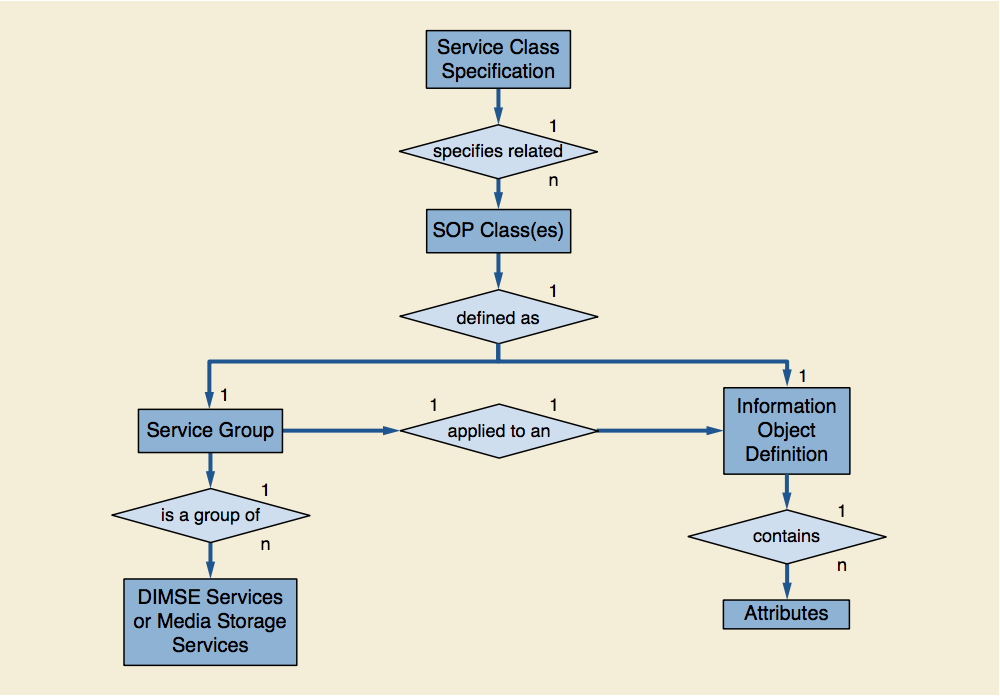
\includegraphics[width = 0.8\hsize]{./figures/DICOMInformationalModel}
\caption{DICOM Informational Model Structure}
\end{figure}

\textbf{Information Object Definition} are abstract object which are intented to represent \textbf{instances of the Real World Model}. More precicely those objects aim at representing classes of element which have some common attributes. \textbf{Information Object Definition}  are made of \textbf{Information Entities (IE)} that stand for the \textbf{Real World Object}. All \textbf{DICOM Object} must at least contains the SOP common module and the four main \textbf{Information Entities}: Patient, Study, Serie and Image.\\

\newline \vspace{5mm}
The \textbf{DIMSE Service Group} specifies operations and notifications that can be applied on an IOD, \textbf{DIMSE} stands for DICOM Message Service Element, \textbf{SOP} are then used for message transfering between \textbf{IOD's}. Together those two element form a \textbf{Service Object Pair (SOP) class} that contains rules and semantics that rule the use of the services.

\newline \vspace{5mm}
When DICOM was created the only instances where images, now other instances that are not images have been introduced but are not of our concern, therefore I will only use the term \textbf{DICOM Images} (DICOM Instance that are Image). As said \textbf{DICOM Images} are \textbf{Information Object Definition}, and must then contain the Image Module besides the four main entieies and the SOP common. This module will contain information about the image itself.

\textbf{DICOM Images} structure is defined on the Figure 2.


\begin{figure}[ht]
\centering
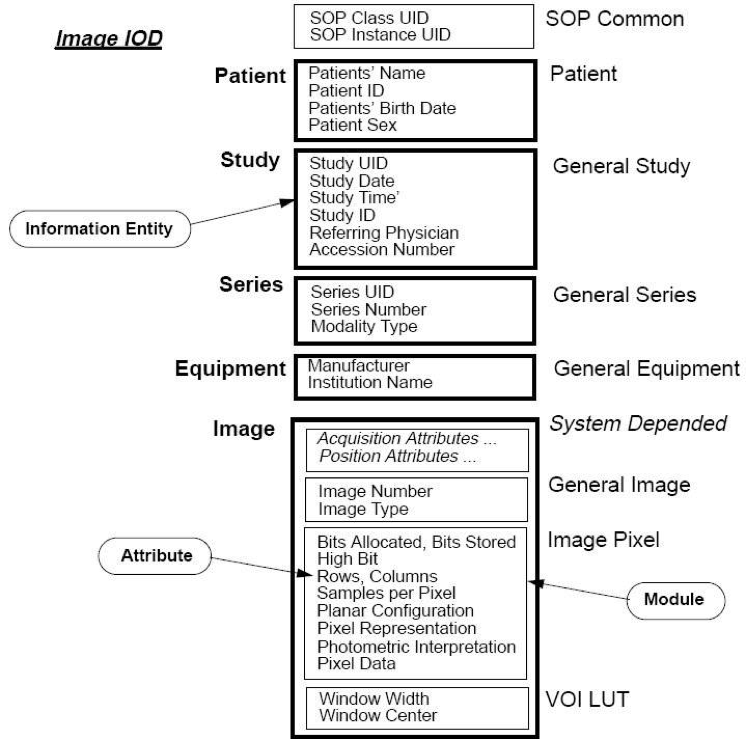
\includegraphics[width = 0.85\hsize]{./figures/ImageIOD}
\caption{Image IOD structure}
\end{figure}

To more extend it is clear on the figure that each Information Entities has an attribute called UID, this stands for \textbf{Unique Identifier}. DICOM uses those identifiers to uniquely defines a wide variety of items to guaranty global uniqueness, mainly among different countries, sites, equimment.


\clearpage

\textbf{3.General File Structure}\\
\newline
DICOM file objects contains informations about the \textbf{DICOM objects of the Real World}, which we know at this stage are held in \textbf{Information Object Definition}. Each DICOM file is composed of two instance: a \textbf{Header} followed by a \textbf{Data Set}.

\begin{figure}[ht]
\centering
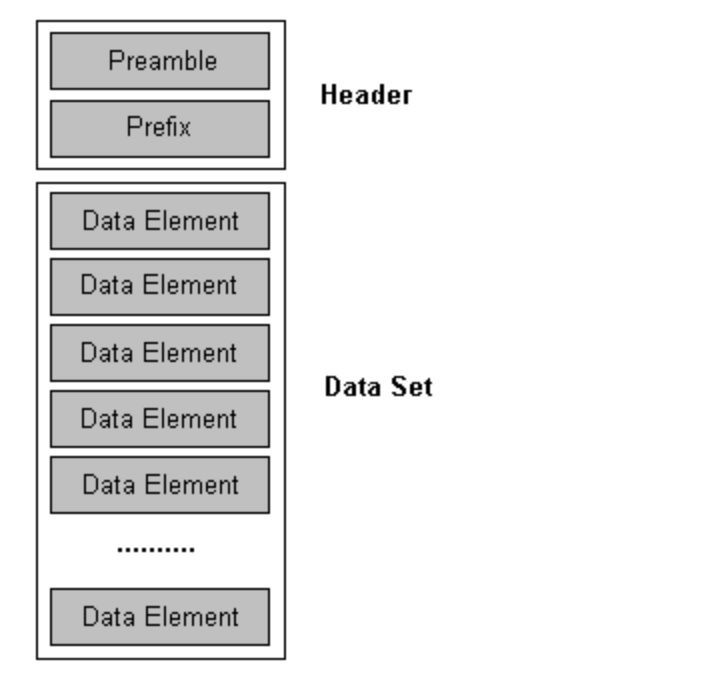
\includegraphics[width = 0.5\hsize]{./figures/DicomFileFormat}
\caption{Basic DICOM File Structure}
\end{figure}


\textbf{The Header} contains 128 bytes preamble (which are all set to zero if it is not used) followed by 4 byte DICOM prefix (DICM). The header is not necessary included in the file but is usefull to make access to data easier, indeed the prefix allows to quickly acknowledge DICOM format. Besides, no structure is required for the preamble.  

\newline \vspace{5mm}
\textbf{The Data Set} is organised as consecutive \textbf{DICOM Data Element} (or Data Attribute) referenced in the DICOM standard. Those Data Element can represent various informations, from the patient name and birth to the pixel image information. More precisely one \textbf{DICOM Data Element} is one unit of information corresponding to an encoded \textbf{Information Object Definition Attribute} defined above.

\newline \vspace{5mm}
\textbf{DICOM Data Element} are “Tag Element” – therefore DICOM can be said to be a tag file format – meaning each element is referenced by a unique \textbf{Tag Number} which define the element and its properties. The Data Set order Data Elements by increasing Tag Number.
Each Data Element is made of the consecutive fields: 
\begin{itemize} 
\item \textbf{Tag Number}: ordered pair of 16bits unsigned integer of the form (gggg,eeee)  representing the Group Number Followed by yhe Element Number.
Eg: (0028,0010): Group Number 0028 correspond to the Image group, Element Number 0010 correspond to the row and especially to the length of the image in pixels 
\item \textbf{Valure Representation}: defines the data type of the element, can be omitted because the Tag Number already implies the data type
\item \textbf{Value Length}: either 16 or 32 bits, defining the length of the following value
\item \textbf{Value Field}: even number of bytes containing the value of the element; the value field can contain the Value Multiplicity, which specified the number of value that can be encoded in the value field. 
\end{itemize}

\begin{figure}[ht]
\centering
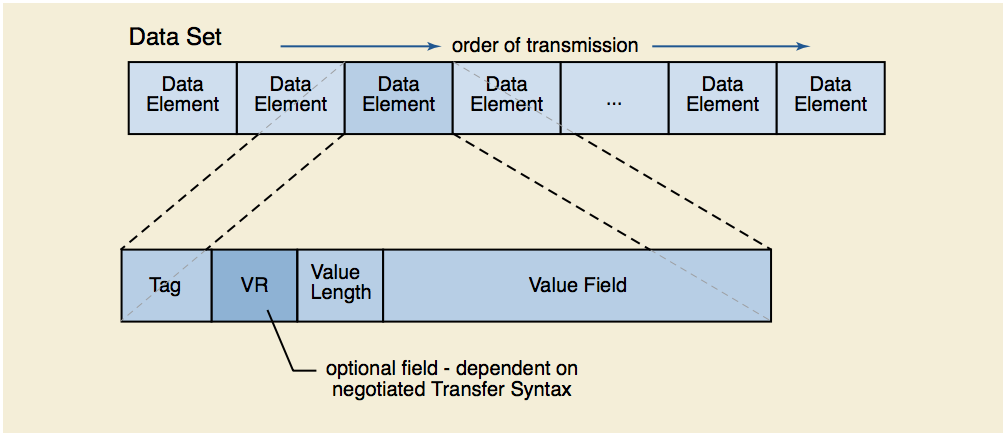
\includegraphics[width = 0.8\hsize]{./figures/DataSetandDataElement}
\caption{Data Set and Data Element structure}
\end{figure}
 

\clearpage

\textbf{4.The DICOMDIR}

\newline \vspace{5mm}
In order the get their DICOM imaging data, patient will be given their DICOM folder. Every basic DICOM folder should contain one element called \textbf{DICOMDIR}. This \textbf{DICOMDIR} is a \textbf{DICOM File Object} containing paths to every DICOM Element that is in the folder; paths are organized within patient, study, serie, image. It also contains the genral informations according the the situation (patient information, study ID, date). The folder might contain other non DICOM element (e.g the report) that won't be recorded by the DICOMDIR. This DICOMDIR is the entry point for my interface and allows me to browse through the DICOM provided file and find path to images.



